

%% this section contains XX problems
%%----------------------------------------


%% Jacobs 5 steps to a 5
%%------------------------------
\element{AP}{
\begin{question}{Jacobs-Q17}
    Which of the following statements about electric potential
        is correct?
    \begin{choices}
        \wrongchoice{A proton experiences a force from a region
            of low potential to a region of high potential.}
      \correctchoice{The potential of a negatively charged
            conductor must be negative.}
        \wrongchoice{If the electric field is zero at point $P$,
            then the electric potential at $P$ must also be zero.}
        \wrongchoice{If the electric potential is zero at point $P$,
            then the electric field at $P$ must also be zero.}
        \wrongchoice{The electric potential with respect to earth
            ground can be less than zero at all points on an
            isolated wire conductor.}
    \end{choices}
\end{question}
}

\element{AP}{
\begin{question}{Jacobs-Q18}
    A uniform electric field points to the right,
        as shown below.
    %\begin{center}
    %    \includegraphics{Jacobs-Q18}
    %\end{center}
    A test charge can be placed at one of three points
        as shown in the above diagram.
    At which point does the test charge experience
        the greatest force?
    \begin{choices}
        \wrongchoice{point A}
        \wrongchoice{point B}
        \wrongchoice{point C}
        \wrongchoice{The charge experiences the greatest
            force at two of the three charges.}
      \correctchoice{The charge experiences the same
            for at all three points.}
    \end{choices}
\end{question}
}

%\element{AP}{
%\begin{question}{Jacobs-Q19}
%    An electron in an electric field is suspended above
%        the Earth's surface.
%    Which of the following diagrams correctly shows the
%        forces acting on this electron?
%    \begin{choices}
%        \wrongchoice{\includegraphics{Jacobs-Q19-A}}
%        \wrongchoice{\includegraphics{Jacobs-Q19-B}}
%      \correctchoice{\includegraphics{Jacobs-Q19-C}}
%        \wrongchoice{\includegraphics{Jacobs-Q19-D}}
%        \wrongchoice{\includegraphics{Jacobs-Q19-E}}
%    \end{choices}
%\end{question}
%}


%% Sample AP 2 Questions
%%------------------------------
\element{AP}{
\begin{question}{AP2-Q02}
    The figure below represents an electric field created by charged objects
        that are not shown.
    The field vectors and the locations $W$ and $Z$ are in the plane of the page.
    \begin{center}
        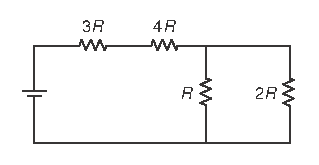
\includegraphics[keepaspectratio]{sample-AP2-Q01}
    \end{center}
    At which location is the electric potential greater?
    \begin{choices}
        \wrongchoice{$W$}
      \correctchoice{$Z$}
        \wrongchoice{Neither; the potential is the same at both locations.}
        \wrongchoice{It cannot be determined without knowing the values of
                     the charges on the objects creating the electric field.}
    \end{choices}
\end{question}
}

\element{AP}{
\begin{question}{AP2-Q03}
    The figure below represents an electric field created by charged objects
        that are not shown.
    The field vectors and the locations $W$ and $Z$ are in the plane of the page.
    \begin{center}
        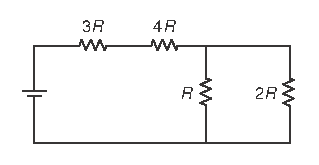
\includegraphics[keepaspectratio]{sample-AP2-Q01}
    \end{center}
    A small charged head held inside the electric field has an electric force
        exerted upon it.
    At which location does the electric force have the greater magnitude?
    \begin{choices}
      \correctchoice{$W$}
        \wrongchoice{$Z$}
        \wrongchoice{Neither; the magnitude of the force is the same at both locations.}
        \wrongchoice{It cannot be determined without knowing the sign of the charge on the bead.}
    \end{choices}
\end{question}
}

%% 2004-APB
%%------------------------------
\element{AP}{
\begin{question}{2004-APB-Q15}
    The hollow metal sphere shown below is positively charged.
    Point $C$ is the center of the sphere and point $P$ is any other
        point within the sphere.
    \begin{center}
        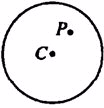
\includegraphics[keepaspectratio]{2004-APB-Q15}
    \end{center}
    Which of the following is true of the electric field at these points?
    \begin{choices}
      \correctchoice{Is is zero at both points.}
        \wrongchoice{It is zero at $C$, but at $P$ is is not zero and is directed inward.}
        \wrongchoice{It is zero at $C$, but at $P$ is is not zero and is directed outward.}
        \wrongchoice{It is zero at $P$, but at $C$ is is not zero.}
        \wrongchoice{It is zero at either point.}
    \end{choices}
\end{question}
}

%% NOTE: Draw vectors with tikz
%\element{AP}{
%\begin{question}{2004-APB-Q19}
%    Charges $-Q$ and $+Q$ are located on the $x$-axis and $y$-axis,
%        respectively, each at a distance $d$ from the origin $O$, as
%        shown below.
%    \begin{center}
%        \includegraphics[keepaspectratio]{2004-APB-Q19}
%    \end{center}
%    What is the direction of the electric field at origin O?
%    \begin{choices}
%        \wrongchoice{\includegraphics[keepaspectratio]{2004-APB-Q18-A}}
%        \wrongchoice{\includegraphics[keepaspectratio]{2004-APB-Q18-B}}
%        \wrongchoice{\includegraphics[keepaspectratio]{2004-APB-Q18-C}}
%      \correctchoice{\includegraphics[keepaspectratio]{2004-APB-Q18-D}}
%        \wrongchoice{\includegraphics[keepaspectratio]{2004-APB-Q18-E}}
%    \end{choices}
%\end{question}
%}

\element{AP}{
\begin{question}{2004-APB-Q20}
    Charges $-Q$ and $+Q$ are located on the $x$-axis and $y$-axis,
        respectively, each at a distance $d$ from the origin $O$, as
        shown below.
    \begin{center}
        \includegraphics[keepaspectratio]{2004-APB-Q19}
    \end{center}
    What is the magnitude of the electric field at origin O?
    \begin{choices}
        \wrongchoice{$\dfrac{kQ}{2d^2}$}
        \wrongchoice{$\dfrac{kQ}{\sqrt{2}d^2}$}
        \wrongchoice{$\dfrac{kQ}{d^2}$}
      \correctchoice{$\dfrac{\sqrt{2}kQ}{d^2}$}
        \wrongchoice{$\dfrac{2kQ}{d^2}$}
    \end{choices}
\end{question}
}

\element{AP}{
\begin{question}{2004-APB-Q21}
    An electron $e$ and a proton $p$ are simultaneously released from rest
        in a uniform electric field $\mathbf{E}$, as shown below.
    \begin{center}
        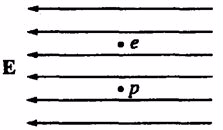
\includegraphics[keepaspectratio]{2004-APB-Q21}
    \end{center}
    Assume that particles are sufficiently far apart so that the only
        force acting on each particle after it is released is that due
        to the electric field.
    At a later time when the particles are still in the field, the electron
        and the proton will have the same
    \begin{choices}
        \wrongchoice{direction of motion}
        \wrongchoice{displacement}
      \correctchoice{magnitude of force acting on them}
        \wrongchoice{speed}
        \wrongchoice{magnitude of acceleration}
    \end{choices}
\end{question}
}

\element{AP}{
\begin{question}{2004-APB-Q45}
    Two large, flat, parallel, conducting plates are \SI{0.04}{\meter}
        apart, as shown below.
    \begin{center}
        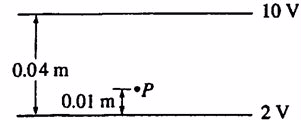
\includegraphics[keepaspectratio]{2004-APB-Q45}
    \end{center}
    The lower plate is at a potential of \SI{2}{\volt} with respect to ground.
    The upper plate is at a potential of \SI{10}{\volt} with respect to ground.
    Point $P$ is located \SI{0.01}{\meter} above the lower plate.
    The electric potential at point $P$ is
    \begin{multicols}{3}
    \begin{choices}
        \wrongchoice{\SI{10}{\volt}}
        \wrongchoice{\SI{8}{\volt}}
        \wrongchoice{\SI{6}{\volt}}
      \correctchoice{\SI{4}{\volt}}
        \wrongchoice{\SI{2}{\volt}}
    \end{choices}
    \end{multicols}
\end{question}
}

\element{AP}{
\begin{question}{2004-APB-Q46}
    Two large, flat, parallel, conducting plates are \SI{0.04}{\meter}
        apart, as shown below.
    \begin{center}
        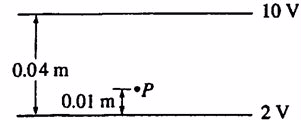
\includegraphics[keepaspectratio]{2004-APB-Q45}
    \end{center}
    The lower plate is at a potential of \SI{2}{\volt} with respect to ground.
    The upper plate is at a potential of \SI{10}{\volt} with respect to ground.
    The magnitude of the electric field at point $P$ is
    \begin{multicols}{3}
    \begin{choices}
        \wrongchoice{\SI{800}{\volt\per\meter}}
        \wrongchoice{\SI{600}{\volt\per\meter}}
        \wrongchoice{\SI{400}{\volt\per\meter}}
      \correctchoice{\SI{200}{\volt\per\meter}}
        \wrongchoice{\SI{100}{\volt\per\meter}}
    \end{choices}
    \end{multicols}
\end{question}
}

\element{AP}{
\begin{question}{2004-APB-Q65}
    A particle of charge $Q$ and mass $m$ is accelerated from rest
        through a potential difference $V$, attaining a kinetic
        energy $K$.
    What is the kinetic energy of particle of charge $2Q$ and
        mass $\tfrac{m}{2}$ that is accelerated from rest through
        the same potential difference.
    \begin{multicols}{3}
    \begin{choices}
        \wrongchoice{$4$}
        \wrongchoice{$2$}
        \wrontchoice{$K$}
      \correctchoice{$2K$}
        \wrongchoice{$4K$}
    \end{choices}
    \end{multicols}
\end{question}
}

\element{AP}{
\begin{question}{2004-APB-Q66}
    The diagram below shows electric field lines in an isolated
        region of space containing two small charges spheres,
        $Y$ and $Z$.
    \begin{center}
        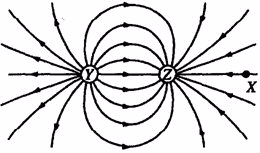
\includegraphics[keepaspectratio]{2004-APB-Q66}
    \end{center}
    Which of the following statements is true?
    \begin{choices}
      \correctchoice{The charge on $Y$ is negative and the charge on $Z$ is positive.}
        \wrongchoice{The strength of the electric field is the same everywhere.}
        \wrongchoice{The electric field is strongest midway between $Y$ and $Z$.}
        \wrongchoice{A small negatively charged object placed at point $X$
            would tend to move toward the right.}
        \wrongchoice{Both charged sphere $Y$ and $Z$ carry charge of the same sign.}
    \end{choices}
\end{question}
}

\element{AP}{
\begin{question}{2004-APB-Q69}
    As shown below, a positively charged particle moves to the right
        without deflection through a pair of charged plates.
    Between the plates are a uniform electric field $E$ of
        magnitude \SI{6.0}{\newton\per\coulomb} and a uniform field
        $B$ of magnitude \SI{2}{\tesla}, directed as shown in
        the figure.
    \begin{center}
        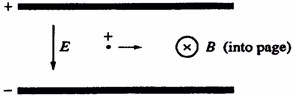
\includegraphics[keepaspectratio]{2004-APB-Q69}
    \end{center}
    The speed of the particle is most nearly
    \begin{multicols}{3}
    \begin{choices}
        \wrongchoice{\SI{0.33}{\meter\per\second}}
        \wrongchoice{\SI{0.66}{\meter\per\second}}
      \correctchoice{\SI{3.0}{\meter\per\second}}
        \wrongchoice{\SI{12}{\meter\per\second}}
        \wrongchoice{\SI{18}{\meter\per\second}}
    \end{choices}
    \end{multicols}
\end{question}
}

\element{AP}{
\begin{question}{2004-APB-Q70}
    A hollow metal sphere \SI{1.0}{\meter} in diameter carries a
        charge of \SI{4.0}{\micro\coulomb}.
    The electric Fidel at a distance of \SI{2.0}{\meter} from
        the center of the sphere is most nearly
    \begin{multicols}{3}
    \begin{choices}
      \correctchoice{\SI{9.0e3}{\newton\per\coulomb}}
        \wrongchoice{\SI{1.8e4}{\newton\per\coulomb}}
        \wrongchoice{\SI{2.4e4}{\newton\per\coulomb}}
        \wrongchoice{\SI{3.6e4}{\newton\per\coulomb}}
        \wrongchoice{\SI{1.4e5}{\newton\per\coulomb}}
    \end{choices}
    \end{multicols}
\end{question}
}

